%! TEX root = /home/duy/TUB/Thesis/latex-source/DiplomarbeitLaTex.tex

\chapter{Evaluation\label{cha:evaluation}}
As we have discussed in the previous chapters, we feed the \acrshort{gan} generated data
to the two-channel Object Classification network in different proportions with respect to
the amount of original data. On one hand, we expect that \acrshort{gan}, especially the
Generator can be a good data generation engine which can help training the classification
task better. On the other hand, we hope that a well-trained classifier could be a good
tool for quantitatively evaluating \acrshort{gan} data.

In this chapter we describe how we evaluate the data generated from \acrshort{gan} using
such a baseline classifier. The basic idea is to implement the two-channel network from
Eitel et al. \cite{eitel} and compare the task's performances between using real data and
using data generated from \acrshort{gan}. Different levels of noise injection are also
used in order to evaluate how the baseline task uses depth and RGB information to make
decisions.

We train the deep classifier in the following settings:

\begin{itemize}
	\item Using the original data with both Depth and RGB information
	\item Using only a part of the original data (in different proportions) with both Depth and
		RGB information
	\item Using a part of the data (in different scales) with both Depth and RGB
		information, the remaining is substituted by \acrshort{gan} generated data
	\item Using the original data but with only RGB information in different proportions
		(10\%, 25\%, and 50\%), to determine the contribution that Depth data adds to the
		learning procedure
\end{itemize}

\section{Learning Curves}
\label{sec:learning_curves}

\acrshort{gan}s are notoriously hard to train, mainly because it does not minimize a
particular scalar function. Fluctuation and Gradient Vanishing of the Discriminator are
common problems, as being described in section \ref{sub:training_gan}. In this project,
fortunately we only face training problems with the Pose-GAN, which is acceptable because
this \acrshort{gan} actually do a much more complicated work than Depth-GAN.

The Depth-GAN's Discriminator-Loss can converge quite early to around 1.4 and becomes a
constant since then, which is a good sign because we have shown in chapter
\ref{cha:relatedwork} that the Optimal Discriminator is at the Absolute Loss of
1.38629436112. It is demonstrated in Figure~\ref{fig:depth_gan_discrim_loss}. As it
already converges, we do not need to perform any regularization here.

\begin{figure}[h!]
	\centering
	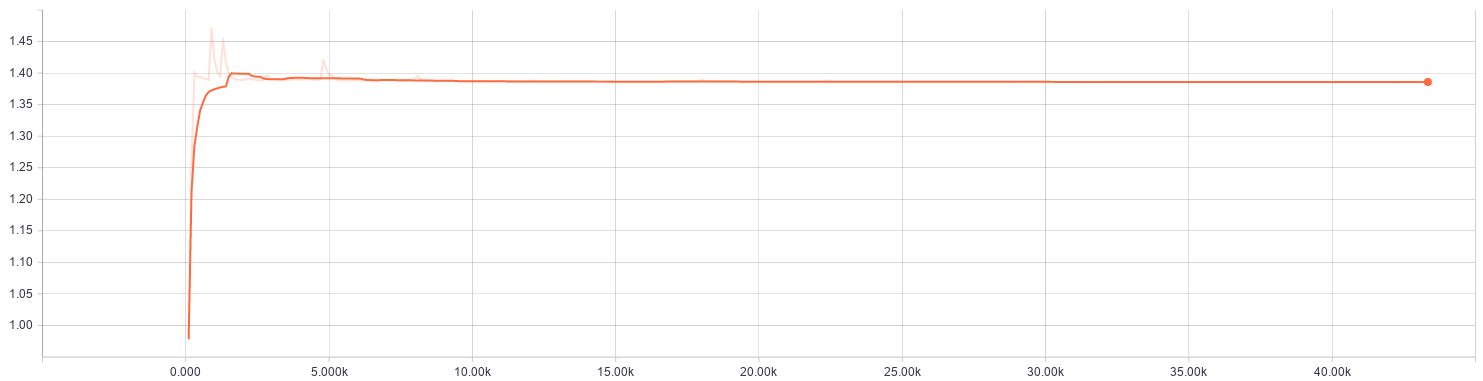
\includegraphics[width=\linewidth]{depth_gan_discrim_loss}
	\caption{The discriminator learning curve of Depth-GAN}
	\label{fig:depth_gan_discrim_loss}
\end{figure}

Things are different for the Pose-GAN, as the Generator has to do a more challenging work
so it is easy to see that the Discriminator can become very good after a short time,
causing Gradient Vanishing. It is very clear in Figure \ref{fig:pose_gan_discrim_loss}. In
the same figure, we can see that the training is much more stabilized after we perform
some regularizations. Particularly, one-sided label smoothing and instance noise injection
are very helpful. Those regularizations help the discriminator loss reaches almost 1.3,
which is much better than previously and is closer to our theoretical Optimal
Discriminator.

\begin{figure}[h!]
	\centering
	
	\begin{subfigure}{\textwidth}
		\begin{center}
			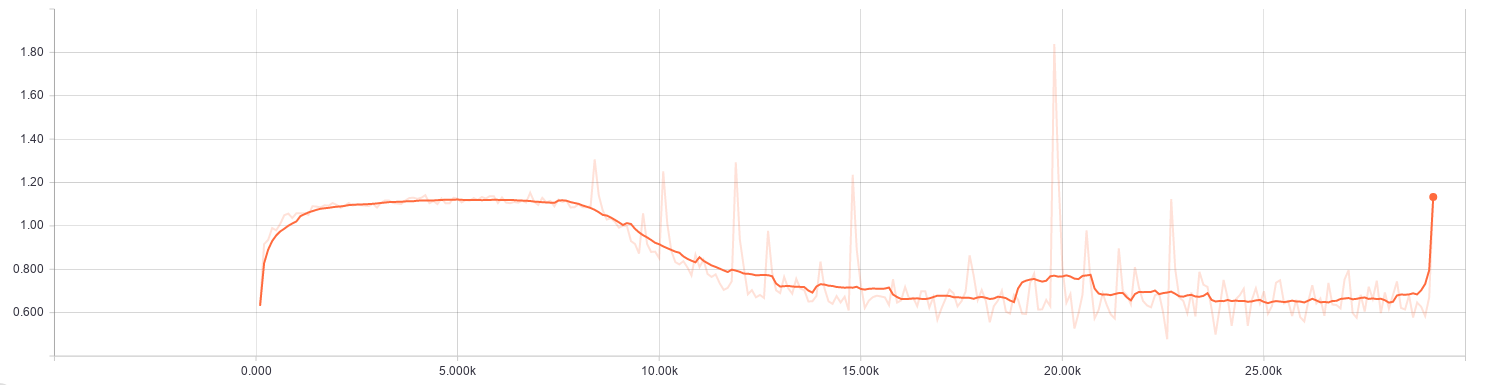
\includegraphics[width=\linewidth]{pose_gan_discrim_loss_no_regularization}
		\end{center}
		\caption{The discriminator learning curve of Pose-GAN, without any regularization}
	\end{subfigure}

	\begin{subfigure}{\textwidth}
		\begin{center}
			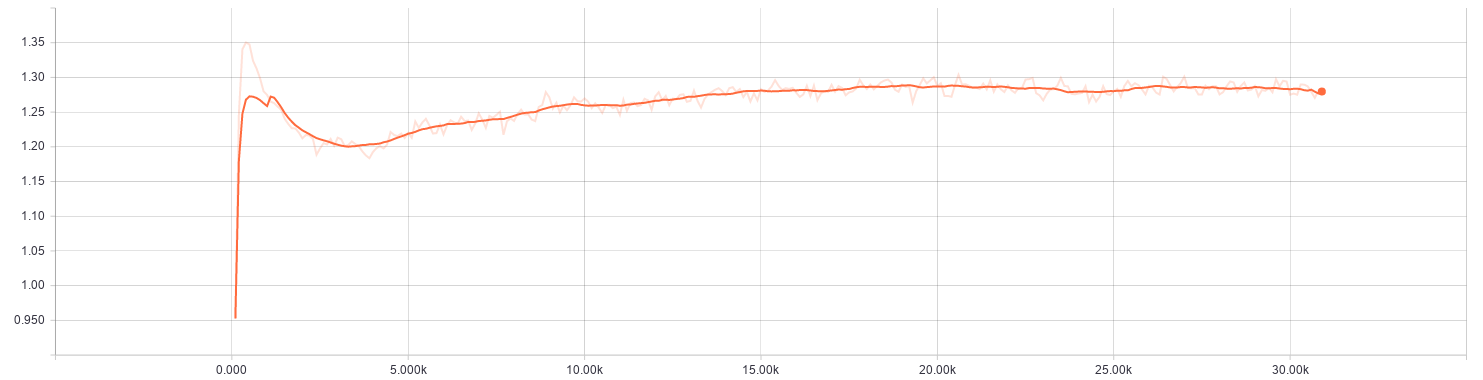
\includegraphics[width=\linewidth]{pose_gan_discrim_loss_regularized}
		\end{center}
		\caption{The discriminator learning curve of Pose-GAN, with slower learning rate,
		input instance noise, and label smoothing}
	\end{subfigure}
	\caption{Pose-GAN's Discriminator Learning Curves}
	\label{fig:pose_gan_discrim_loss}
\end{figure}

\section{Results}
\label{sec:results}

Before going to quantitative measurements, it is worthy to take a look as what our
\acrshort{gan}s produce.

\subsection{Depth-GAN}
\label{sub:depth_gan}

In Figure~\ref{fig:gan_depth}, 5 random samples from 5 random categories in the dataset
are the outputs from our Depth-GAN in Evaluation Mode, which means the corresponding
\acrshort{gan} did not see those samples in the training process.  We show the results
from all the three versions that we trained: Using 50\%, 25\% and 10\% of training data.
The depth maps are all colorized using the jet color-map for visualization purpose. It is
easy to see that the \acrshort{gan} produces very reasonable depth maps with a smooth
range of values. It is also important to see that when we reduce the amount of training
data from 50\% to 25\% and 10\%, the quality of the synthesized depth maps also noticeably
reduces. The latter Depth-GANs produce images with more noise; but they still have decent
details. This is understandable as we have explained in section
\ref{sec:train_test_split}.

Taking a look at those maps, we can see that the \acrshort{gan} does learn some trivial
knowledge. For instance, the bottom pixels tend to be closer to the sensor than the pixels
at the top of the image; and when there is a sharp edge or a sudden change of color
patterns, there is usually an object placed on top of another. We can clearly see the
second property in the sample of the fruits and the keyboard in Figure~\ref{fig:gan_depth}.

In these sample outputs from our Depth-GAN, we also see another popular advantage of
\acrshort{gan} which is already discussed in some other works \cite{gan, cogan, pix2pix}.
That is, the edges in the synthesized images are very sharp. If we instead minimized a
squared loss function for example, we could expect a much more blurry outcome. It is also
one of the reasons that using common scalar error functions such as \acrshort{mse} is not
a good way to evaluate \acrshort{gan}s' results.

\clearpage

\begin{figure}[h!]
	\centering
	\begin{subfigure}{0.8\textwidth}
		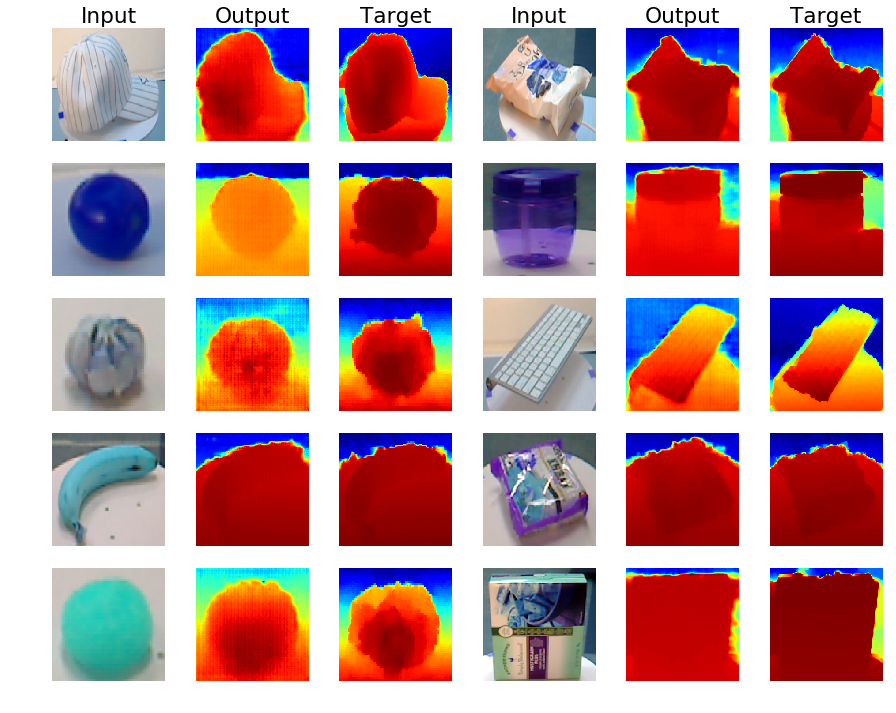
\includegraphics[width=\textwidth]{gan_depth_samples_50}
		\caption{Depth-GAN trained with 50\% data} 
	\end{subfigure}
	\begin{subfigure}{0.49\textwidth}
		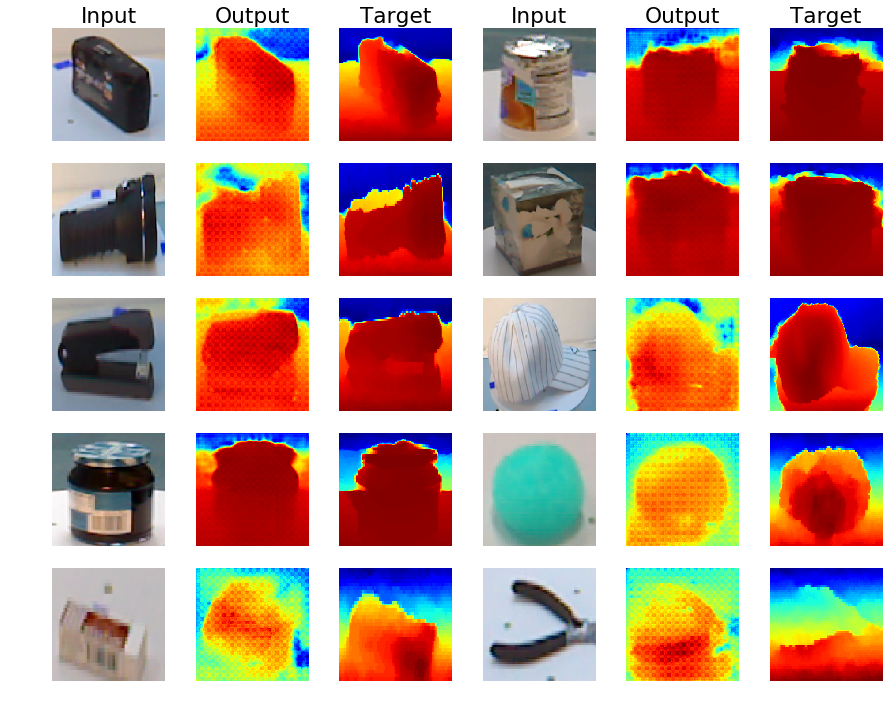
\includegraphics[width=\textwidth]{gan_depth_samples_25}
		\caption{Depth-GAN trained with 25\% data} 
	\end{subfigure}
	\begin{subfigure}{0.49\textwidth}
		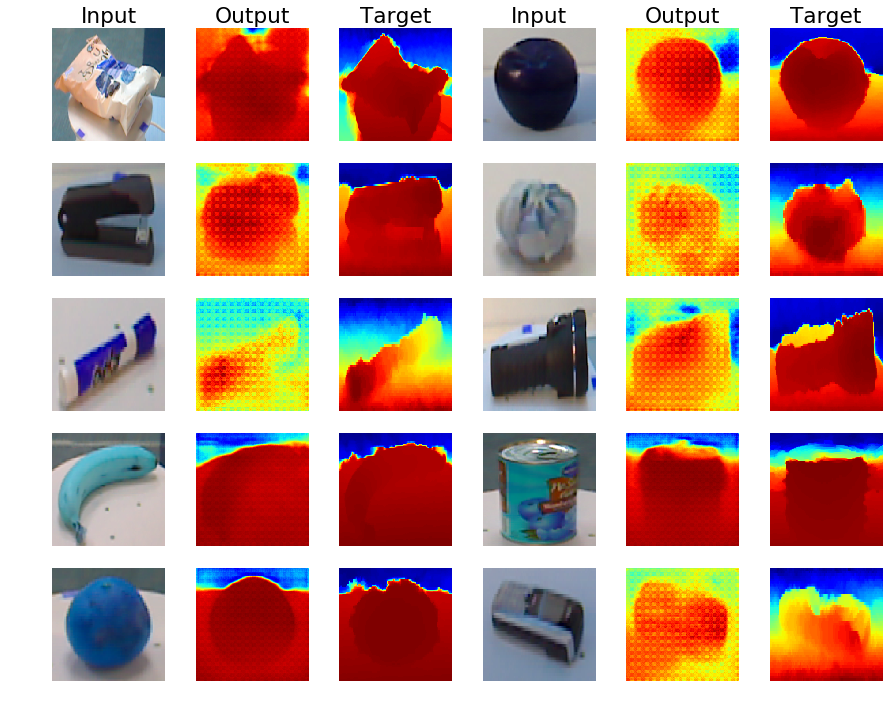
\includegraphics[width=\textwidth]{gan_depth_samples_10}
		\caption{Depth-GAN trained with 10\% data} 
	\end{subfigure}
	
	%\centering
	%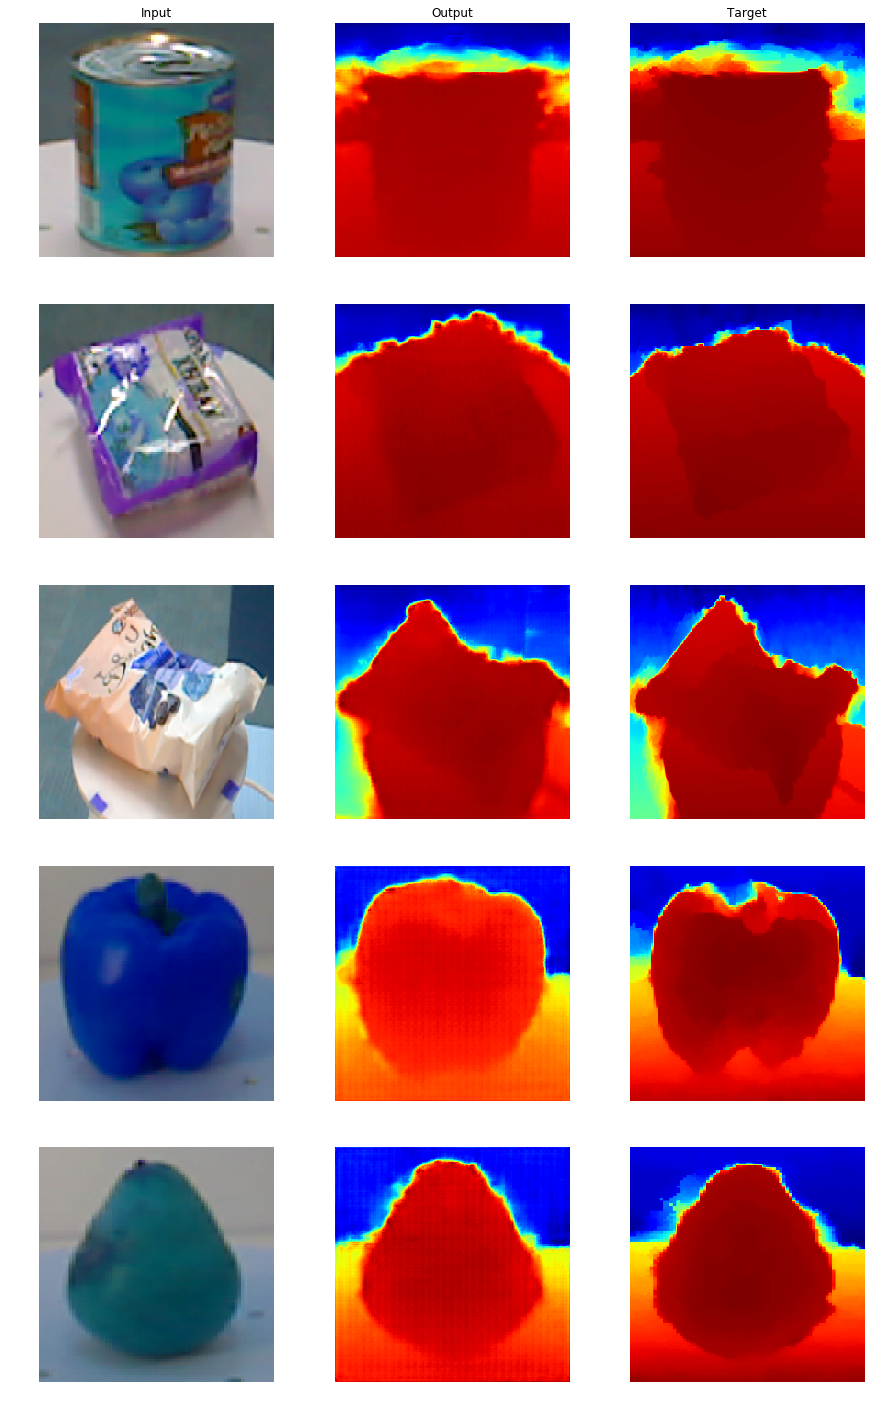
\includegraphics[width=0.72\linewidth]{gan_depth_samples}
	\caption{Some generated samples from Depth-GAN. The Output and the Target are colorized using the jet color-map.}
	\label{fig:gan_depth}
\end{figure}

\subsection{Pose-GAN}
\label{sub:pose_gan}

Similarly to the section above, Figure~\ref{fig:gan_pose_samples} shows some examples
generated from our Pose-GAN. Visually, the Outputs do not look too bad, some of them, such
as the cell phone, the flashlight and the boxes, are clearly rotated. However, the details
are clearly not optimal, and it works better with round-shape objects because they look
the same in different points of view. The overall feeling is that, the synthesized objects
are acceptable in terms of human eyes, but there is a certain level of noise in those
images, which means the Generator is still somehow confused with the given
condition/input.

\begin{figure}[h!]
	\centering
	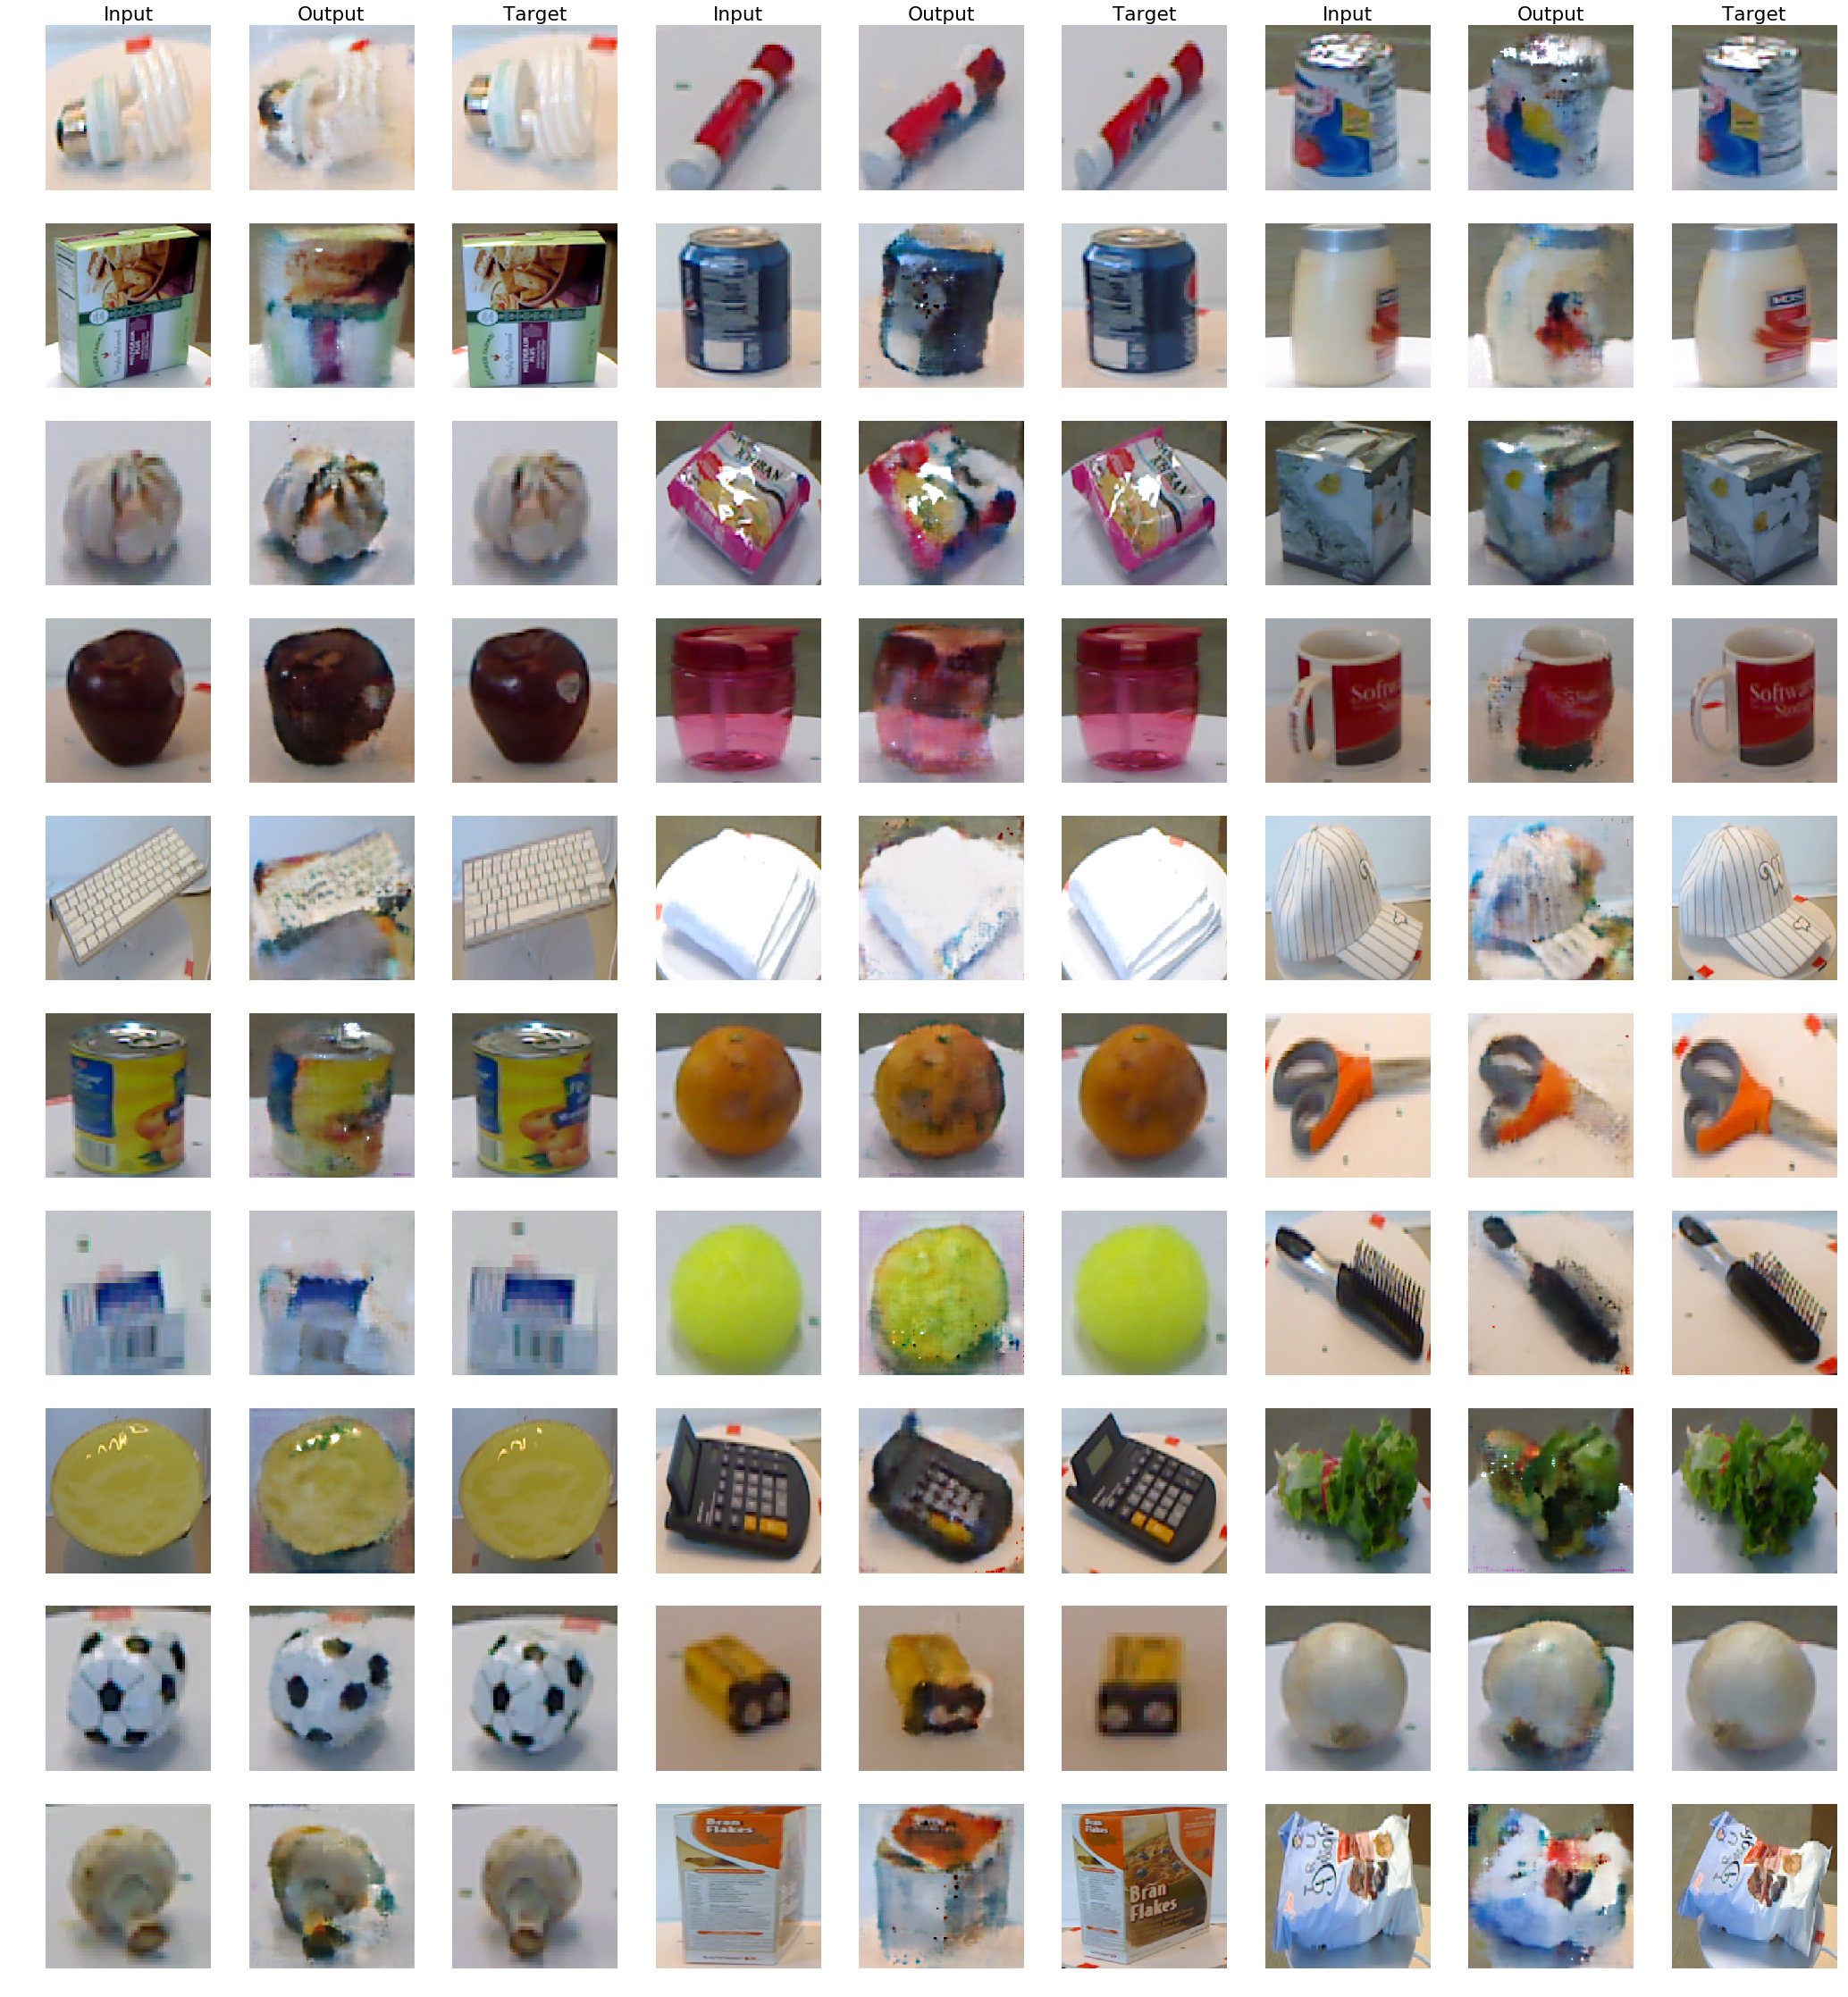
\includegraphics[width=\linewidth]{gan_pose_samples}
	\caption{Some generated samples from Pose-GAN trained with 50\% data. Note: The actual
		input is a 4-D image with the 4th dimension being the Depth-map, here we show only the
	RGB frame.}
	\label{fig:gan_pose_samples}
\end{figure}

\section{Performance of Depth-GAN Data}

In the first experiment, we try to reproduce Eitel et al. \cite{eitel}. We can
see the plotted results in Figure \ref{fig:eitel_accuracies}.

In general, we can see that \acrshort{gan} has good contribution in the classification
performance. It is worth mentioning that the transfer learning technique works very well,
so we still have the accuracies more than 80\% even when we use only 10\% of the data. It
is also expected to see the accuracies drop when we use only RGB data for training the
network, but the difference is only a few percentages, which is an indication that the
contribution of depth information is low in this training procedure. It is not a surprise
because the RGB channels themselves have already achieved a very high accuracy
(approximately 90\%). However, as other works also have shown \cite{eitel, alexandre},
depth information does help improving classification on \acrfull{cnn} when combining with
RGB, our experiment also follows that trend where all the accuracies using depth data are
higher in average than the corresponding results without depth.

\begin{table}[h!]
	\centering
	\caption{Dependent T-Test (rounded) results between different training experiments.
		For each block, Depth-GAN data is added to the training set (the
		right-hand-side numbers) and there is one experiment with only RGB data. All
		accuracies are compared with the result batch trained by the corresponding amount
		of original data. All values lower than 0.05 are highlighted.}
	\label{tab:t_test}
	\begin{tabular}{|l|l|l|}
		\hline
		Experiments      & p-values                        & Compared To            \\ \hline
		50 with only RGB & \textbf{0.0001} & \multirow{5}{*}{50-0}  \\ \cline{1-2}
		50-50            & \textbf{0.0156}   &                        \\ \cline{1-2}
		50-40            & \textbf{0.0220}   &                        \\ \cline{1-2}
		50-30            & 0.2173 			 &                        \\ \cline{1-2}
		50-20            & 0.9369 			 &                        \\ \hline
		25 with only RGB & \textbf{4.7233e-05} & \multirow{2}{*}{25-0}  \\ \cline{1-2}
		25-75            & \textbf{2.4228e-05} &                        \\ \hline
		10 with only RGB & \textbf{1.2940e-05}  & \multirow{2}{*}{10-0}  \\ \cline{1-2}
		10-90            & \textbf{2.7698e-06} &                        \\ \hline
		50-50            & 0.1249				& \multirow{3}{*}{100-0} \\ \cline{1-2}
		25-75            & 0.1803				&                        \\ \cline{1-2}
		10-90            & \textbf{0.0006}  	&                        \\ \hline
	\end{tabular}
\end{table}

It can be seen from Figure~\ref{fig:eitel_accuracies} that the absolute mean accuracies of
the classification noticeably increases when we add the \acrshort{gan} synthesized data to
the training set. In order to verify that, we run a Dependent T-test for the relevant
experiments to see if the accuracies significantly change or not. The reason why we choose
the Dependent Test is that our statistics are the results of the same experiment
(Evaluating a Deep Neural Network) under different settings. So using the Test for Paired
Samples is reasonable.

\begin{figure}[h!]
	\caption{Classification accuracies on Washington Dataset in different settings,
		trained and tested in 10 stratified random splits. The left number in a pair indicates
		the proportion of real data, and the right number indicates the proportion of synthesized
	data added.}
	\centering
	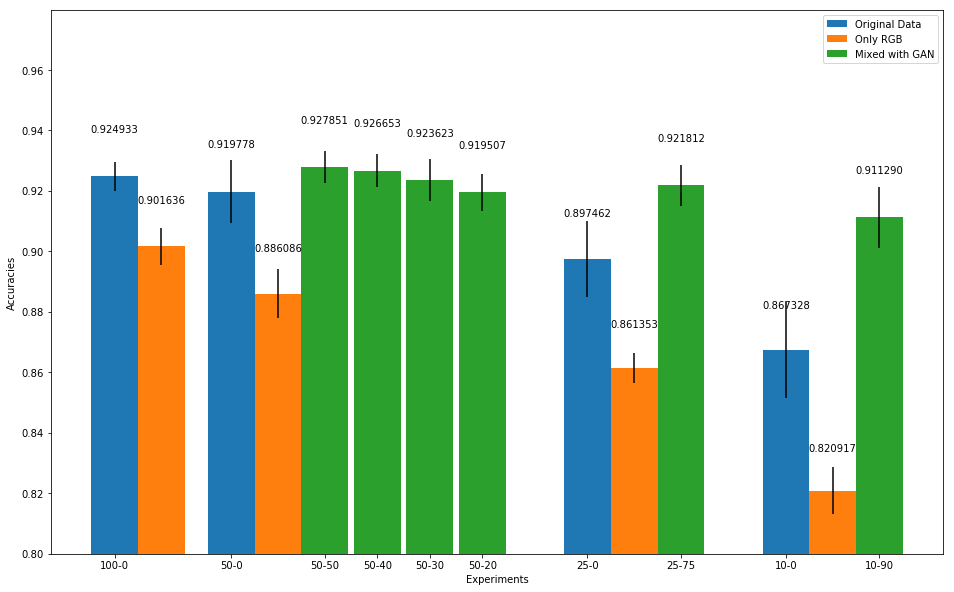
\includegraphics[width=0.9\textwidth]{img/eitel_accuracies}
	\label{fig:eitel_accuracies}
\end{figure}

\begin{figure}[h!]
	\centering
	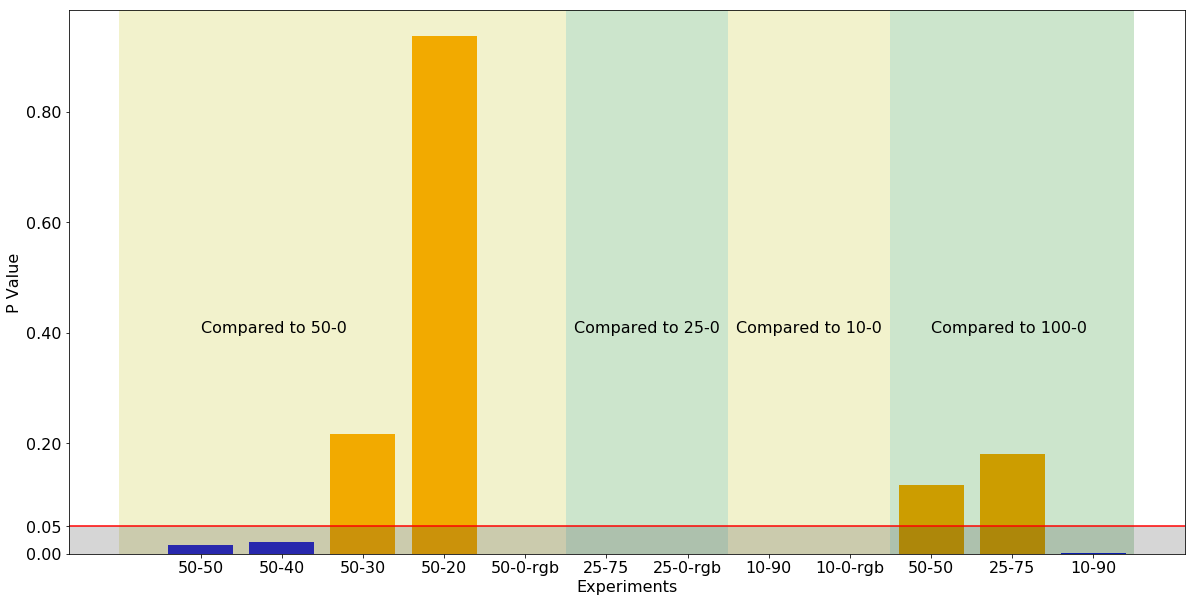
\includegraphics[width=0.9\linewidth]{t_test_plot}
	\caption{Visualization of table \ref{tab:t_test}. The blue bars are lower
	and the orange bars are higher than 0.05. 
	%Most of the important proportions of \acrshort{gan} data produce significantly
	%different accuracies (higher).  When comparing with the whole original data, only the
	%10-90 case yields a significantly different accuracy (lower). 
	Note: Some values are too small that they do not show clearly in this plot (see table
	\ref{tab:t_test}), but the important point is they are much smaller than 0.05 (the red
line)}
\label{fig:t_test_plot}
\end{figure}

In Figure~\ref{fig:eitel_accuracies}, there are 14 different experiments. We definitely do
not test every pair of experiments there, but instead only compare the results involving
\acrshort{gan} (the green bars) with the results with original data (the blue bars). In
this way, we would like to verify if training with \acrshort{gan} data is significantly
better than training without it. A significant level of 0.05 is used in all the tests. The
null hypothesis is "the 2 set of results are equal". In this statistical test, we combine
both the T-test and the mean accuracies plot in \ref{fig:eitel_accuracies} to reach a  
conclusion. If the test says that we can reject the null hypothesis, we conclude that the
one having higher mean is significantly better than the one having lower mean.

We can see in Table \ref{tab:t_test}, or even more clearly in the visualized version in
Figure \ref{fig:t_test_plot}, the T-test p-values for the experiments plotted in
Figure~\ref{fig:eitel_accuracies}. Based on those plots, we can conclude which strategies
significantly improve the classification training procedure.

In the case of 50\% of the original data, following the significant level of 0.05, we can
reject the null hypothesis for the case of 50-50, 50-40, and 50 with only RGB, meaning
they are significantly different from the results of 50-0.  As the plot in
Figure~\ref{fig:eitel_accuracies} shows higher mean values for 50-50 and 50-40 and lower
value for 50 with only RGB, it is reasonable to conclude that adding those proportions of
\acrshort{gan} data improves training the classifier significantly, and adding depth data
to the training indeed adds important values to the network. In this case we add
incremental amounts of \acrshort{gan} data (20\%, 30\% and 40\%) to see the trend of
\acrshort{gan}'s contribution. The accuracy plot \ref{fig:eitel_accuracies}, together with
the T-test results \ref{tab:t_test}, shows a clear incremental contribution with respect
to the amount of \acrshort{gan} data.

For the cases of 25\% and 10\% of original data, we only experiment with the full amount of
\acrshort{gan} data. The p-values are even more significantly lower than 0.05, indicating
that the results we have by adding 75\% and 10\%, respectively, of the training data from
our \acrshort{gan} are strongly better than the accuracies without them. The p-values of
the training with only RGB still shows the same trend with the 50\% case, saying that it
is meaningful to use Depth data in training our Object Classifier.

In addition, we also compare the results from full-combination results (i.e. 50-50, 25-75
and 10-90) with the accuracies of the classifier trained from 100\% of the original data
from the Washington RGB-D dataset. The p-values are in the last 3 rows of Table
\ref{tab:t_test}. We can only reject the null hypothesis in the case of 10-90.
Statistically, we cannot conclude that our accuracies with 50-50 and 25-75 are equal to
that of 100-0, but we have a strong base for saying that our \acrshort{gan} data can train
a comparable classifier with the optimal case. Only the 10-90 data shows a significantly
lower accuracies than 100-0, which is understandable as this Depth-GAN is trained with
only 10\% of the data which is probably not enough for it to capture the whole data
space. It is also one of the limitations of our experiment strategies, which is already
discussed in section \ref{sec:train_test_split}.


\section{Contribution of Depth Data in the Baseline Classifier}
In the previous section, we have already seen that the depth data from \acrshort{gan} helps
improving the classification performance in an RGB-Depth two-channel Deep Neural Network.
However, it was still not clear how much Depth Data contributes to the task. This is
important because if the network only learns from RGB data, our previous results do not
make too much sense and do not prove that our Depth-GAN is learning good Depth
Representations. A good news is, the previous experiments also revealed that the accuracies
achieved using only the RGB channels are significantly lower than with Depth involved. 

In this section, we would like to clarify how Depth contributes to the learning process by
doing a noise injection to the evaluation procedure of the Object Classification network.
We add Gaussian noises with mean 0 and standard deviations of 5, 10, 15, 20, and 40 respectively 
to the RGB, Depth, and both RGB and Depth channels of the Test Set and observe the
behaviors of the Deep Network during the Evaluation process. 

\begin{figure}[h!]
	\centering
	\begin{subfigure}{0.32\textwidth}
		\centering
		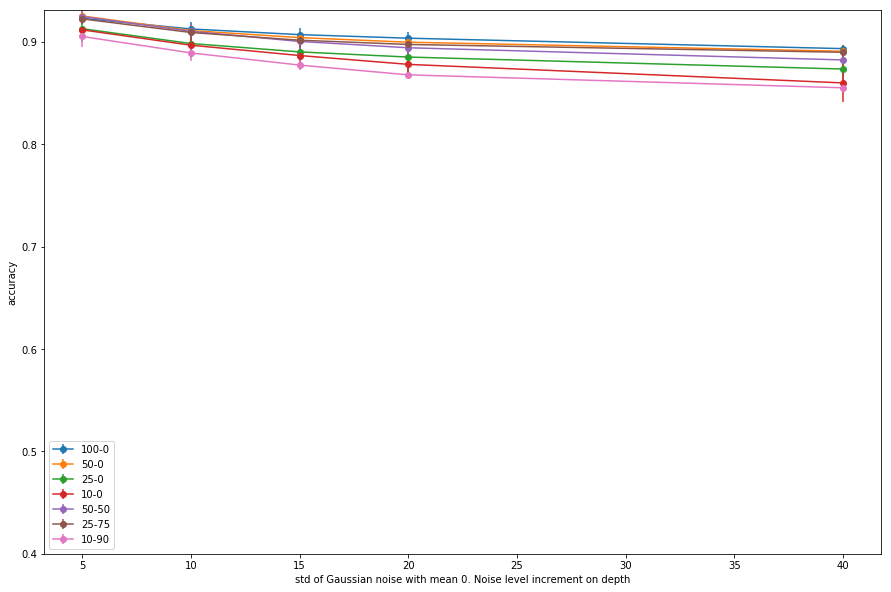
\includegraphics[width=\textwidth]{img/noise_injection_depth}
		\caption{Adding noises to depth}
	\end{subfigure}
	\begin{subfigure}{0.32\textwidth}
		\centering
		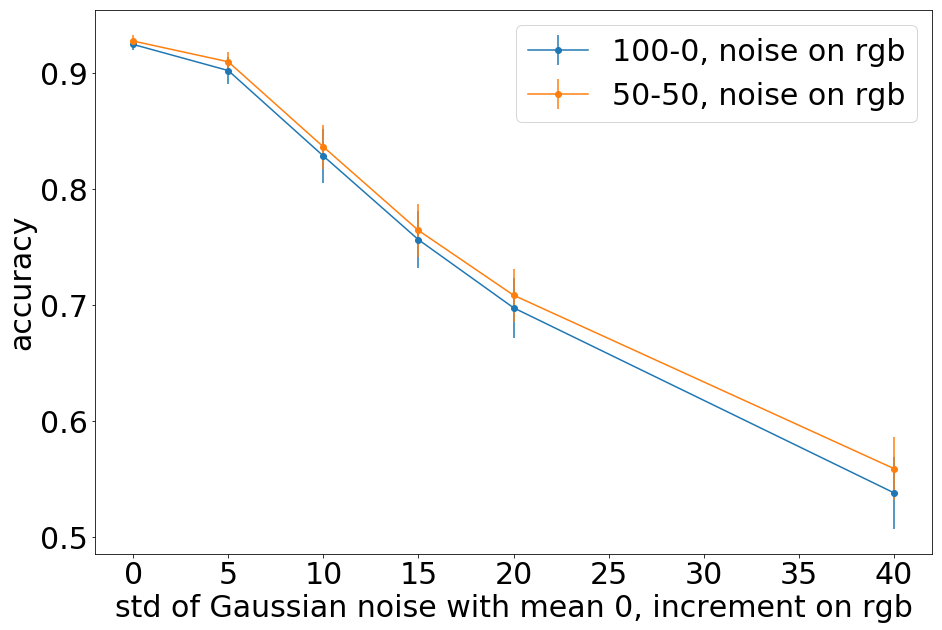
\includegraphics[width=\textwidth]{img/noise_injection_rgb}
		\caption{Adding noises to RGB}
	\end{subfigure}
	\begin{subfigure}{0.32\textwidth}
		\centering
		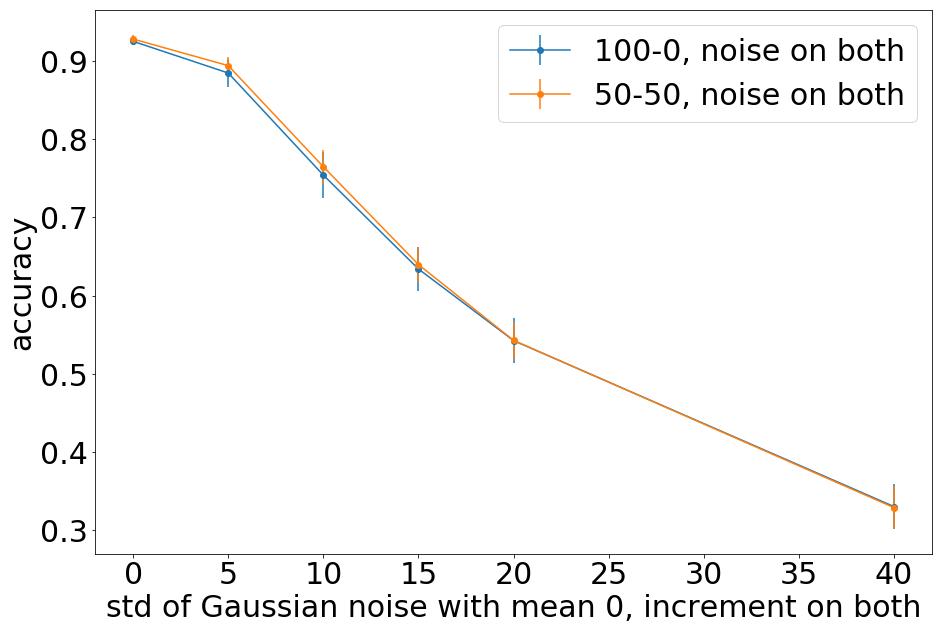
\includegraphics[width=\textwidth]{img/noise_injection_both}
		\caption{Adding noises to both channels}
		\label{subfig:noise_both}
	\end{subfigure}
	\caption{Noise Injection experiments. When adding noise to Depth, we experiment with
	the original training set (100-0) and all the combinations involving synthesized
depth. In the other two noise experiments, we perform them on only the original training
set and the strongest combination of synthesized depth (50-50) as we expect similar
behaviors from the combinations of synthesized depth. Note: The scales of 3 figures are
different.}
	\label{fig:noise_injection}
\end{figure}

Figure~\ref{fig:noise_injection} summarizes the behaviors of different experiments. There
are clearly different trends between adding noises to Depth and adding noises to RGB. When
adding noises to the RGB channels, the decrement of accuracies is more linear, whereas
when adding noises to the Depth channel, it is only linear up to a standard deviation of
20. Between 20 and 40, the decrement clearly vanishes, indicating that we are reaching a
limit of Depth contribution. In the same scale of noises, the behavior of the network when
we add noises to the RGB channels is different, it is almost a straight line from 5 to 40.
Figure~\ref{subfig:noise_both} shows a very similar pattern (to RGB) when we add noises to
both channels, which means RGB are the dominant channels here. In addition,
Figure~\ref{fig:noise_injection_2_channels} compares the rate of decrement when putting
the noise injection behaviors of the same dataset (50-50) in the same scale. The injection
to RGB is much steeper than the injection to Depth.

\begin{figure}[h!]
	\centering
	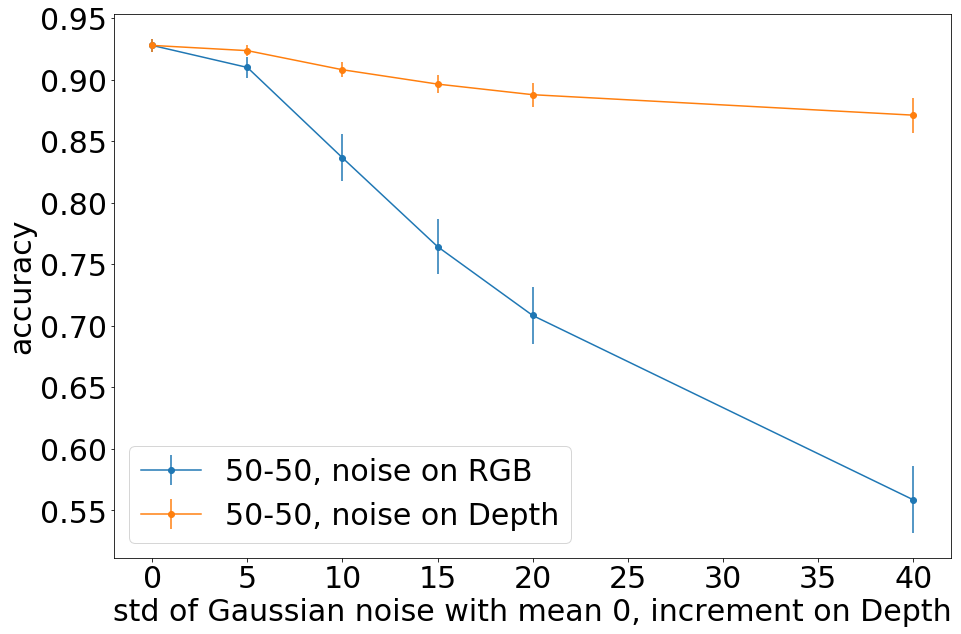
\includegraphics[width=0.9\linewidth]{noise_injection_2_separate_channels}
	\caption{Noise Injection on RGB and Depth separately, performing on the same
	synthesized depth combination and visualized in the same scale.}
	\label{fig:noise_injection_2_channels}
\end{figure}

\section{Performance of Pose-GAN Data \label{sec:performance_pose}}

For Pose-GAN, we train the baseline classifier with only the 50-50 proportion. Although
the resulting images look reasonable, they are still not perfect. There are many blurry
details, especially in complex objects such as the cereal box with textures and the comb,
or in objects with very similar color with the background such as the towel and the rubber
eraser. Therefore, it is not a surprise that we achieve only an accuracy of 66\% when
training the object classifier with the \acrshort{gan} data. As this is a very bad overall
accuracy and because of time limitation, we do not go further to perform the same
experiments as what we do with Depth-GAN. However, it is probably a good idea to look at
the category-wise accuracies to see which categories are easy for the \acrshort{gan} to learn
and which are not.

\begin{figure}[h!]
	\centering
	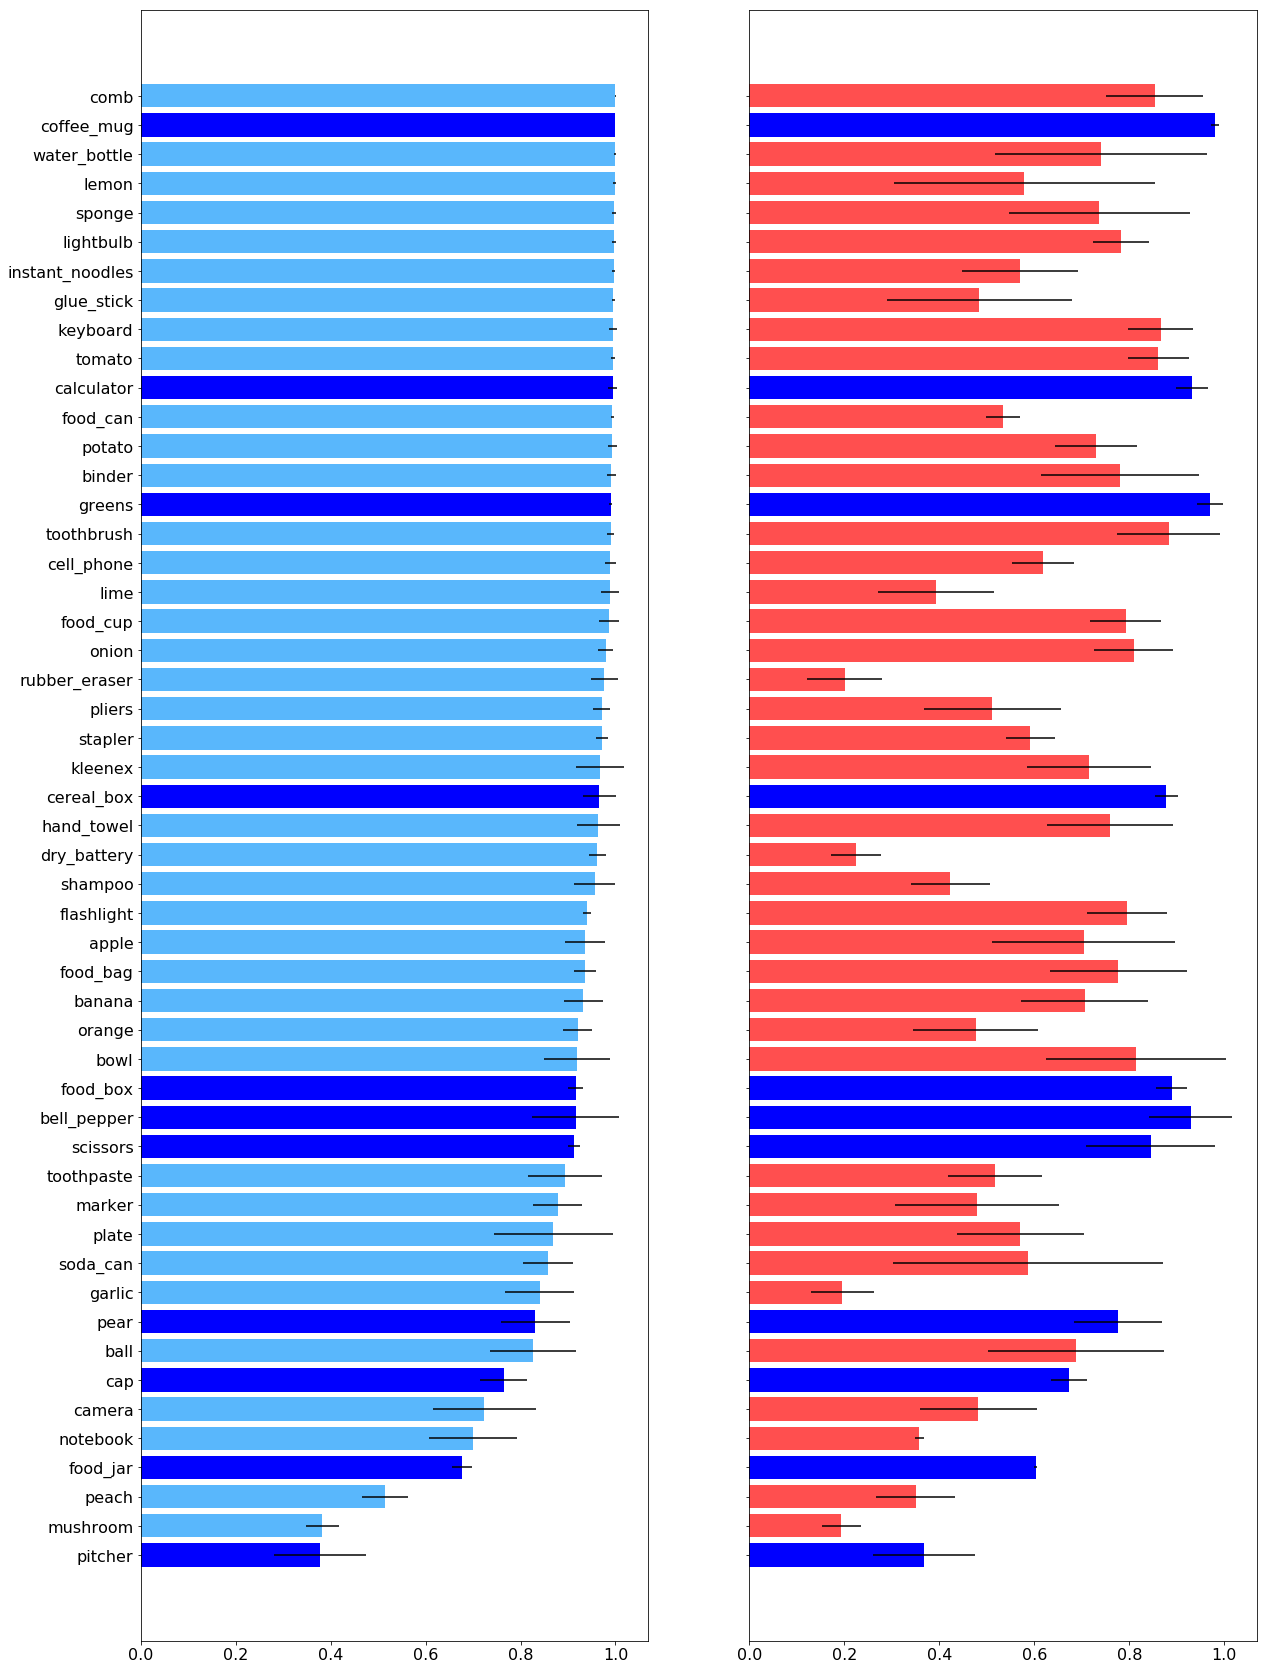
\includegraphics[width=\linewidth]{pose_gan_accuracies}
	\caption{Category-wise accuracies of the original data (Left) and Pose-GAN Data in
		50-50 proportion (Right). All the categories that the Pose-GAN performance is
		acceptable are highlighted in blue. By "acceptable" we mean that the accuracies is within
	a 0.1 error bound compared with the original data.}
	\label{fig:pose_gan_accuracies}
\end{figure}

In Figure~\ref{fig:pose_gan_accuracies}, only a few categories are
as-well-or-better classified using the data from the Pose-GAN, which means this
\acrshort{gan} is still not good enough to capture the entire 3D space representation,
although most of the synthesized RGB images are still distinguishable by human eyes (see
Figure \ref{fig:gan_pose_samples}).

We demonstrate some categories that the Pose-GAN performs quite well in
Figure~\ref{fig:acceptable}. Most of the synthesized objects still have problems with
complex details, but some of them are very fine. The calculator, for instance, is
well-rotated and can be clearly detected by human eyes; and the details such as the keypad
are still adequate. The Bell Pepper is almost perfect, but it is a round object so it is
easier for the Generator to learn. The Coffee Mug is successfully rotated, but loses all
the sharp textures.

\begin{figure}[h!]
	\centering
	\begin{subfigure}{0.32\textwidth}
		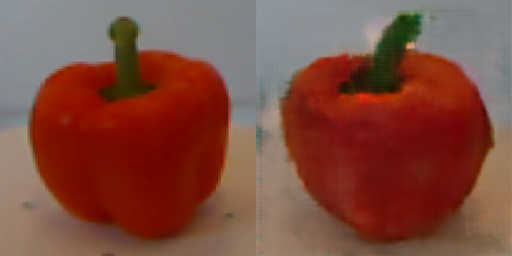
\includegraphics[width=\textwidth]{acceptable/bell_pepper_1_1_12}
		\caption{Bell Pepper}
	\end{subfigure}
	\begin{subfigure}{0.32\textwidth}
		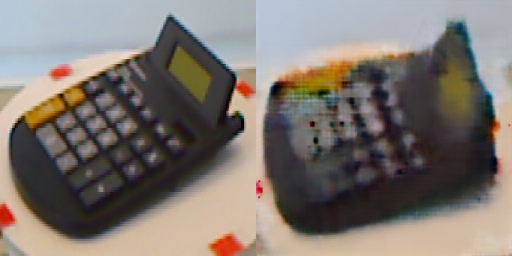
\includegraphics[width=\textwidth]{acceptable/calculator_2_1_2}
		\caption{Calculator}
	\end{subfigure} 
	\begin{subfigure}{0.32\textwidth}
		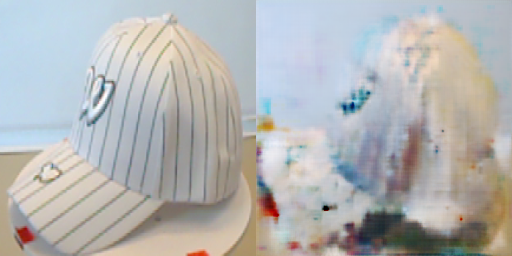
\includegraphics[width=\textwidth]{acceptable/cap_1_1_2}
		\caption{Cap}
	\end{subfigure} 
	\begin{subfigure}{0.32\textwidth}
		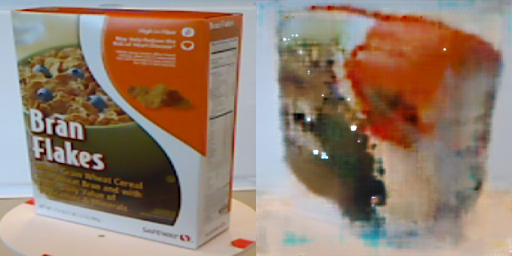
\includegraphics[width=\textwidth]{acceptable/cereal_box_1_1_2}
		\caption{Cereal Box}
	\end{subfigure} 
	\begin{subfigure}{0.32\textwidth}
		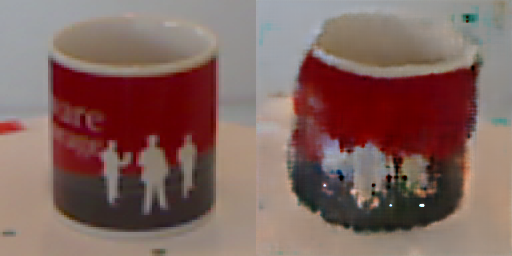
\includegraphics[width=\textwidth]{acceptable/coffee_mug_1_1_5}
		\caption{Coffee Mug}
	\end{subfigure} 
	\begin{subfigure}{0.32\textwidth}
		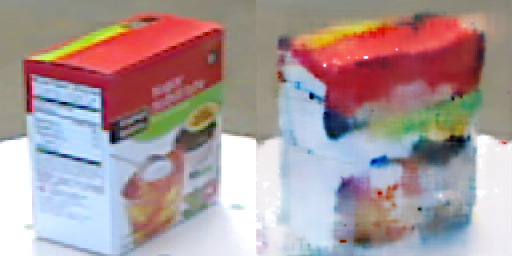
\includegraphics[width=\textwidth]{acceptable/food_box_1_1_14}
		\caption{Food Box}
	\end{subfigure} 
	\begin{subfigure}{0.32\textwidth}
		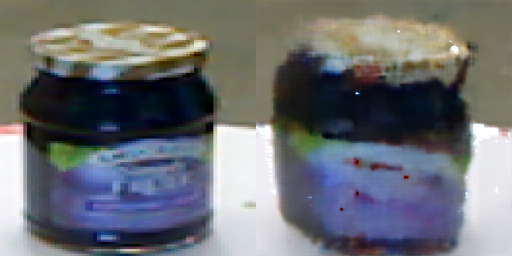
\includegraphics[width=\textwidth]{acceptable/food_jar_1_1_14}
		\caption{Food Jar}
	\end{subfigure} 
	\begin{subfigure}{0.32\textwidth}
		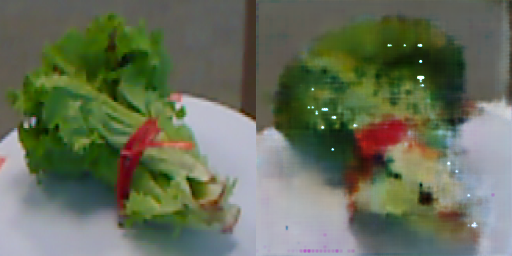
\includegraphics[width=\textwidth]{acceptable/greens_1_1_5}
		\caption{Greens}
	\end{subfigure} 
	\begin{subfigure}{0.32\textwidth}
		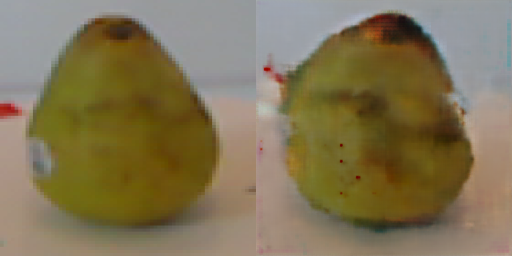
\includegraphics[width=\textwidth]{acceptable/pear_1_1_3}
		\caption{Pear}
	\end{subfigure} 
	\begin{subfigure}{0.32\textwidth}
		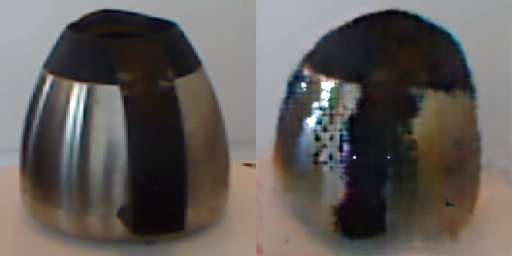
\includegraphics[width=\textwidth]{acceptable/pitcher_2_1_2}
		\caption{Pitcher}
	\end{subfigure} 
	\begin{subfigure}{0.32\textwidth}
		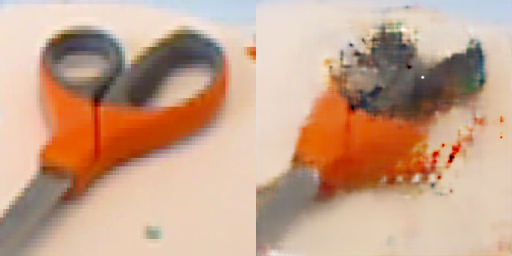
\includegraphics[width=\textwidth]{acceptable/scissors_1_1_2}
		\caption{Scissors}
	\end{subfigure} 
	
	\caption{Samples from the categories in which the synthesized objects produce
		acceptable accuracies, in figure \ref{fig:pose_gan_accuracies}. On the left are
	the original objects, on the right are the rotated pose produced by Pose-GAN.}
	\label{fig:acceptable}
\end{figure}

\begin{figure}[h!]
	\centering
	\begin{subfigure}{0.32\textwidth}
		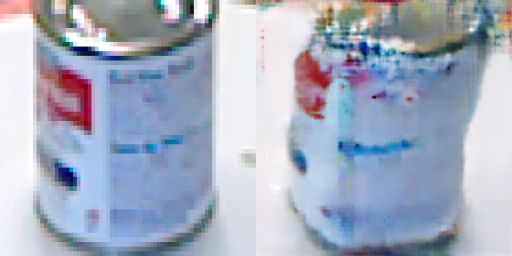
\includegraphics[width=0.8\linewidth]{not_acceptable/food_can_1_1_14}
		\caption{Food Can}
	\end{subfigure}
	\begin{subfigure}{0.32\textwidth}
		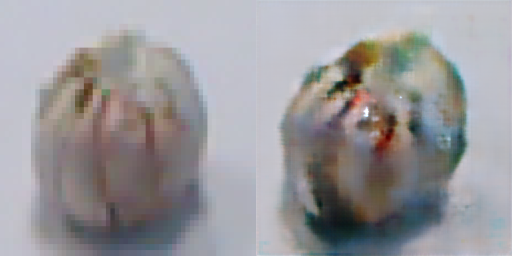
\includegraphics[width=0.8\linewidth]{not_acceptable/garlic_1_1_15}
		\caption{Garlic}
	\end{subfigure}
	\begin{subfigure}{0.32\textwidth}
		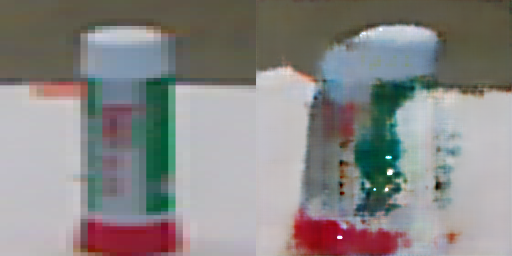
\includegraphics[width=0.8\linewidth]{not_acceptable/glue_stick_1_1_2}
		\caption{Glue Stick}
	\end{subfigure}
	\begin{subfigure}{0.32\textwidth}
		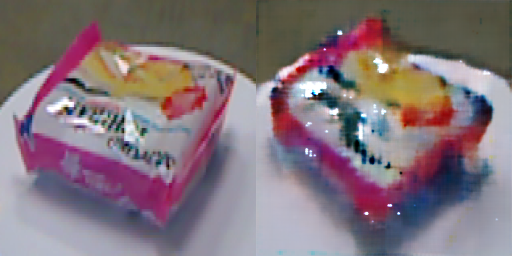
\includegraphics[width=0.8\linewidth]{not_acceptable/instant_noodles_2_1_14}
		\caption{Instant Noodles}
	\end{subfigure}
	\begin{subfigure}{0.32\textwidth}
		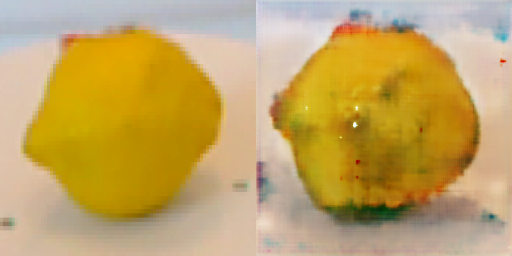
\includegraphics[width=0.8\linewidth]{not_acceptable/lemon_1_1_2}
		\caption{Lemon}
	\end{subfigure}
	\begin{subfigure}{0.32\textwidth}
		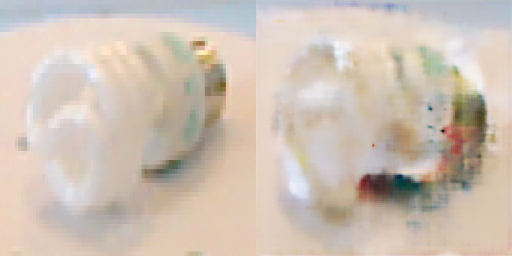
\includegraphics[width=0.8\linewidth]{not_acceptable/lightbulb_1_1_2}
		\caption{Light Bulb}
	\end{subfigure}
	\begin{subfigure}{0.32\textwidth}
		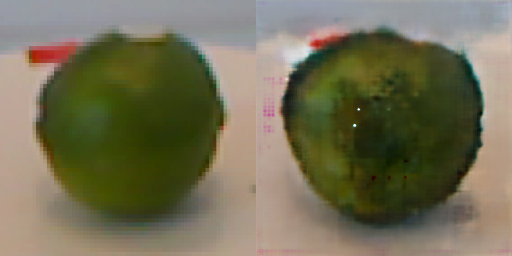
\includegraphics[width=0.8\linewidth]{not_acceptable/lime_1_1_8}
		\caption{Lime}
	\end{subfigure}
	\begin{subfigure}{0.32\textwidth}
		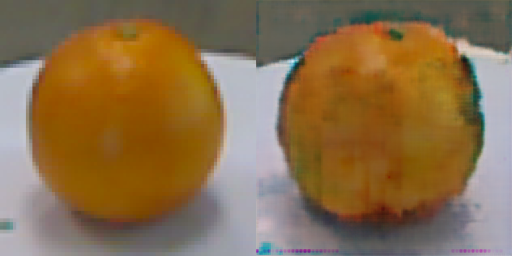
\includegraphics[width=0.8\linewidth]{not_acceptable/orange_1_1_2}
		\caption{Orange}
	\end{subfigure}
	\begin{subfigure}{0.32\textwidth}
		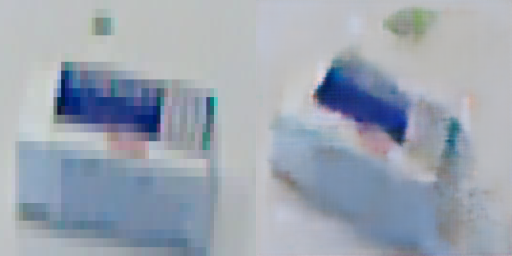
\includegraphics[width=0.8\linewidth]{not_acceptable/rubber_eraser_1_1_2}
		\caption{Rubber Eraser}
	\end{subfigure}
	\begin{subfigure}{0.32\textwidth}
		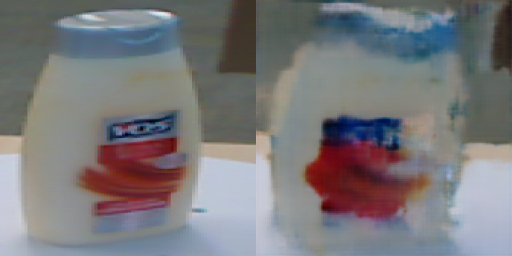
\includegraphics[width=0.8\linewidth]{not_acceptable/shampoo_1_2_4}
		\caption{Shampoo}
	\end{subfigure}
	\begin{subfigure}{0.32\textwidth}
		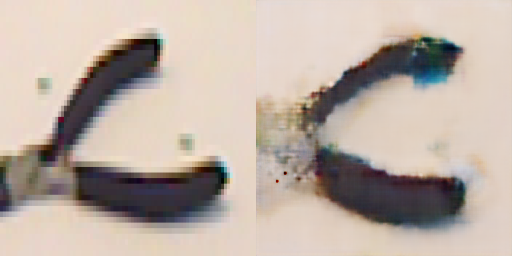
\includegraphics[width=0.8\linewidth]{not_acceptable/pliers_2_1_3}
		\caption{Pliers}
	\end{subfigure}
	\begin{subfigure}{0.32\textwidth}
		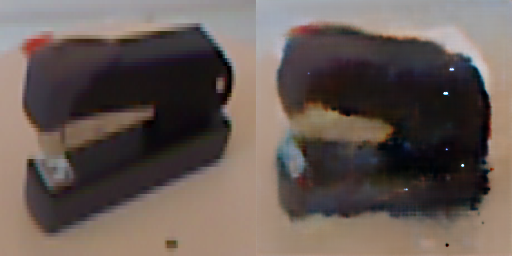
\includegraphics[width=0.8\linewidth]{not_acceptable/stapler_2_1_2}
		\caption{Stapler}
	\end{subfigure}
	
	\caption{Samples from the categories in which the synthesized objects does not produce
		good results in figure \ref{fig:pose_gan_accuracies}.}
	\label{fig:not_acceptable}
\end{figure}

On the contrary, Figure~\ref{fig:not_acceptable} shows some examples of the objects
behaving much worse in the classifier than the original data.  Among the failed ones, only
The Light Bulb and the Glue Stick are indeed bad. They do not have a clear shape and are
not clearly distinguishable from the background. The rest of them still look quite nice,
such as the Instant Noodles, the Stapler and the Rubber Eraser. The Shampoo and the Food
Can are not as good as the two above, but are still better, or at least comparable to the
Cap and the Food Box in Figure~\ref{fig:acceptable}. An observed phenomenon is that
regardless of how we train the Pose-GAN, the classification results of those categories
are still equally bad, although the visual outcomes do improve noticeably as we apply more
regularization tricks. This raises an interesting question on why the classifier fails to
correctly recognize the synthesized images while they still look very good to human eyes;
and at the same time performs greatly with the real counterparts. More work might need to
be done in order to find the reason why they behave differently while sharing similar
appearance qualities. 

Because we remove 17 categories from the Pose-GAN's training set as being mentioned in
section \ref{sub:training_gan}, we also try to make it a fairer game by also removing the
same categories from the training and test sets of the classifier. However, the results of
the remaining categories show no differences from what we have discussed above.
